\section{Operación}
\label{anexo:operacion}

A continuación se describen los pasos a seguir para operar 
de manera correcta la planta.

\subsection{Acciones iniciales y carga del programa}

\begin{enumerate}
 \item Controlar el nivel de agua en los tanques según el anexo \ref{anexo:puestaEnMarcha}.
 \item Controlar que las válvulas manuales estén en su correcta
 posición según el anexo \ref{anexo:puestaEnMarcha}.
 \item Conectar el aire a presión según el anexo \ref{anexo:puestaEnMarcha}.
 \item Conectar la planta a la red eléctrica.
 \item Activar en interruptor termomagnético ubicado dentro del tablero
 eléctrico.
 \item Conectar la planta con la computadora mediante el cable cable RS-485 
 con adaptación a RS-232. Puede ser necesario utilizar un adaptador RS-232/USB.
 \item Abrir el programa del \gls{plc} denominado {\color{red}(nombre del programa)} 
 con el Software Twido Soft. Este programa se encuentra en el DVD adjunto a este 
 informe.
 \item Conectarse al \gls{plc} como se indica en la imagen \ref{img:twidosoft}.
 \item Cargar el programa en el \gls{plc}, imagen \ref{img:twidosoftcargar}.
 \item Poner a correr el programa, imagen\ref{img:twidosoftrun}.
 \item Desconectarse del \gls{plc}, imagen \ref{img:twidosoftdesc}.
\end{enumerate}
\todo{imagen del programa y colocar el nombre definitivo del programa}


\begin{figure}[ht!]
	\centering
	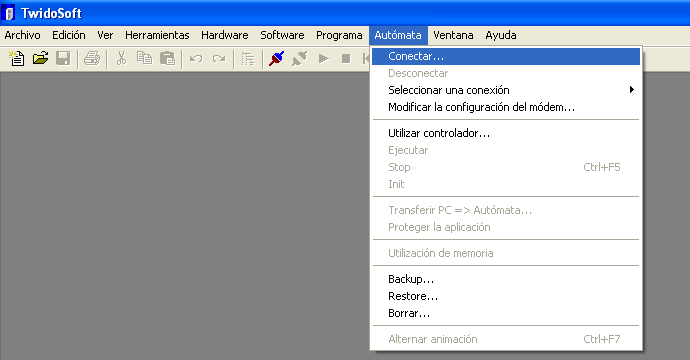
\includegraphics[scale=0.5]{Anexos/images/twidosoft.PNG}
	\caption{Esquema de la división del tiempo}
	\label{img:twidosoft}
\end{figure}

\begin{figure}[ht!]
	\centering
	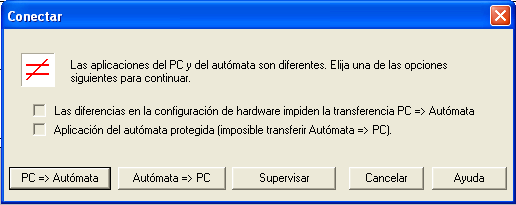
\includegraphics[scale=0.3]{Anexos/images/twidosoftcargar.PNG}
	\caption{Esquema de la división del tiempo}
	\label{img:twidosoftcargar}
\end{figure}

\begin{figure}[ht!]
	\centering
	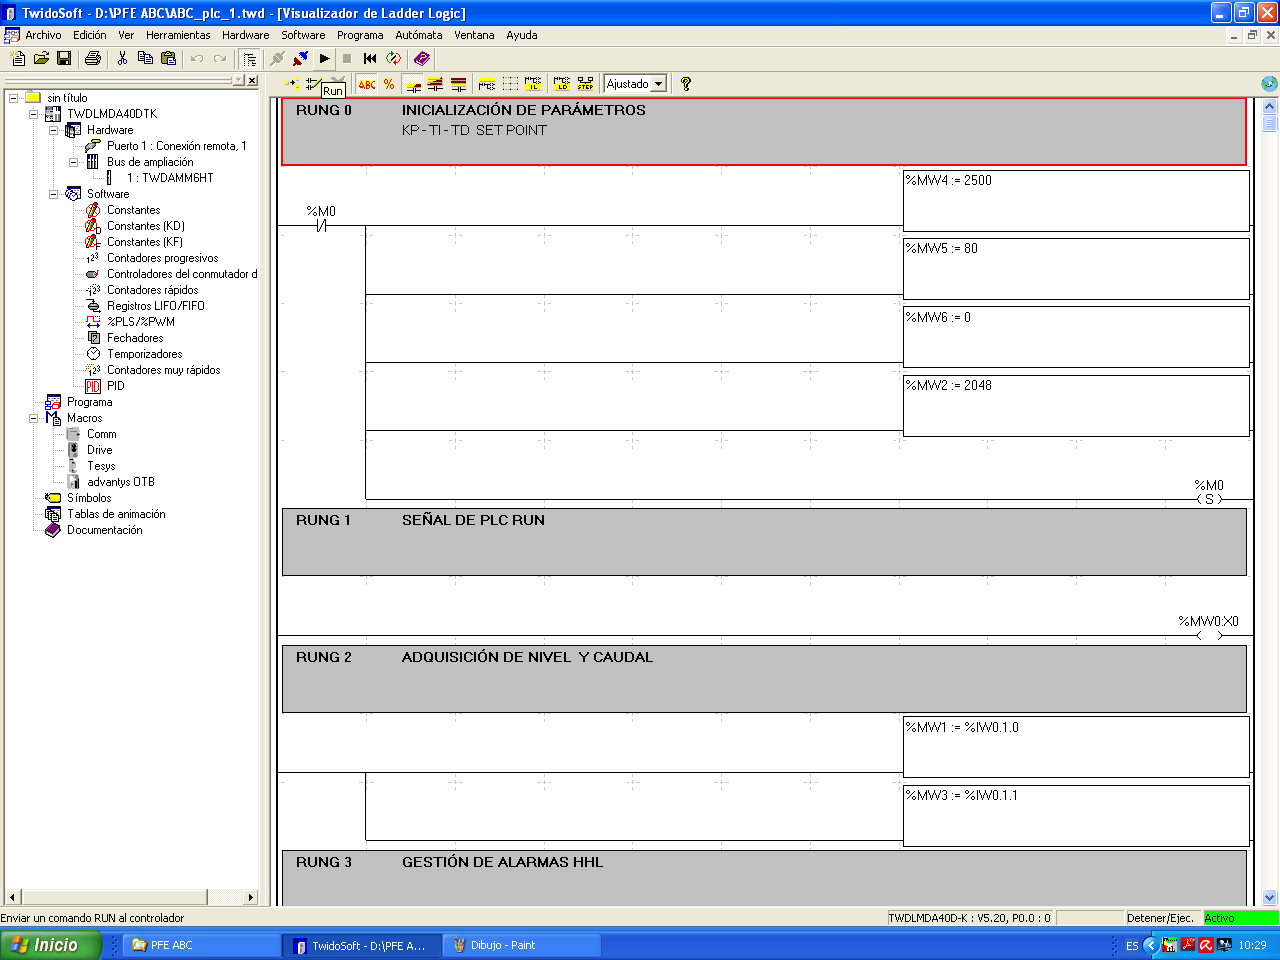
\includegraphics[scale=0.3]{Anexos/images/twidosoftrun.PNG}
	\caption{Esquema de la división del tiempo}
	\label{img:twidosoftrun}
\end{figure}

\begin{figure}[ht!]
	\centering
	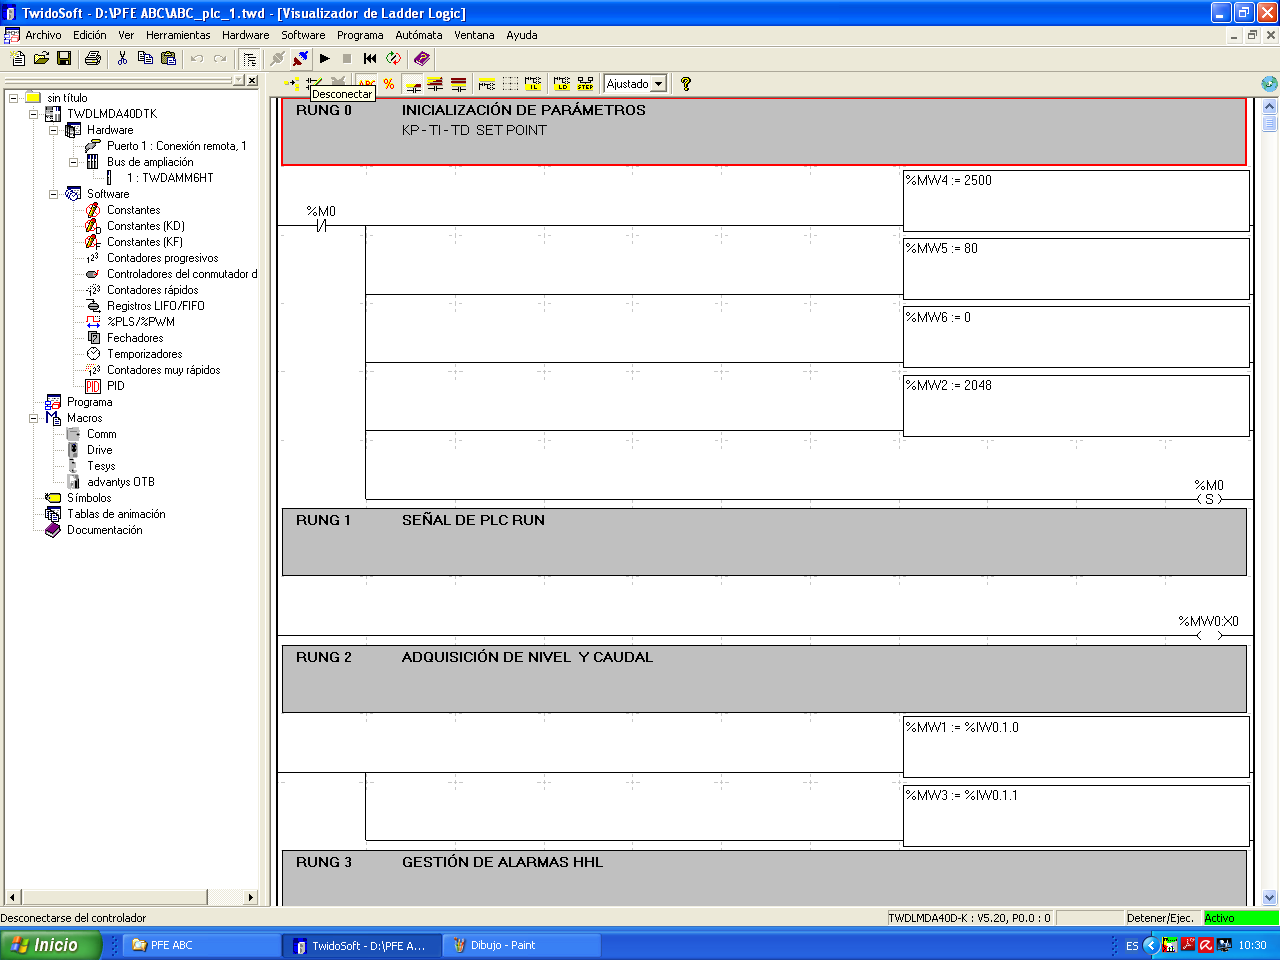
\includegraphics[scale=0.3]{Anexos/images/twidosoftdesc.PNG}
	\caption{Esquema de la división del tiempo}
	\label{img:twidosoftdesc}
\end{figure}

\subsection{SCADA}